\documentclass[letterpaper,13pt,addpoints]{exam}
\usepackage[utf8]{inputenc}
\usepackage[english]{babel}
\usepackage{listings}
\usepackage{graphicx}
\usepackage{xcolor}
\usepackage[top=1in, bottom=1in, left=0.75in, right=0.75in]{geometry}
\usepackage{amsmath,amssymb}

\definecolor{codegreen}{rgb}{0,0.6,0}
\definecolor{codegray}{rgb}{0.5,0.5,0.5}
\definecolor{codepurple}{rgb}{0.58,0,0.82}
\definecolor{backcolour}{rgb}{0.95,0.95,0.92}

\lstdefinestyle{mystyle}{
    commentstyle=\color{codegreen},
    keywordstyle=\color{blue},
    stringstyle=\color{codepurple},
    basicstyle=\ttfamily\small,
    breakatwhitespace=false,
    breaklines=true,
    captionpos=b,
    keepspaces=true,
    showspaces=false,
    showstringspaces=false,
    showtabs=false,
    tabsize=2
}

\newcommand{\university}{UNIVERSITY OF IBRA}
\newcommand{\faculty}{Department of Numeracy, Computation, and Probability}
\newcommand{\class}{CSC108H5 F}
\newcommand{\examnum}{(Not) Penultimate Examination}
\newcommand{\content}{Introduction to Computer Programming}
\newcommand{\examdate}{2023/12/08}
\newcommand{\timelimit}{Good Luck.}

\pagestyle{headandfoot}
\firstpageheader{}{}{}
\firstpagefooter{}{Page \thepage\ of \numpages}{}
\runningheader{\class}{\examnum}{\examdate}
\runningheadrule
\runningfooter{}{Page \thepage\ of \numpages}{}

\begin{document}

\title{\Large \textbf{\university\\ \faculty\\
        \bigskip
        \class -- \examnum \\ \content}}
\author{Instructors: Themba, Ibrahim}
\date{Duration: Good Luck.\\ Aids Allowed: God Himself.\\ \examdate}
\maketitle
\begin{center}
    \makebox[12cm]{\textbf{Name}:\ \hrulefill}
    \medskip
    \makebox[12cm]{\textbf{Student Number}:\ \hrulefill}
\end{center}

% Hey copilot how do I make a square border around text?
\begin{center}
    \fbox{\parbox{6.5in}{\textit{The University of Ibra and you, as a student, share a
                commitment to academic integrity. You are reminded that you may be charged with
                an academic offence for possessing any unauthorized aids during the writing of
                an exam. Clear, sealable, faraday bags have been provided for all mythical
                devices, including but not limited to: telepathic communication headsets, time
                machines, polygraph machines, magic wands, Miraculouses, and any other
                supernatural or futuristic devices that could potentially aid in unfair
                advantages during examinations. Please turn off all devices, seal them in the
                bag provided, and place the bag under your desk for the duration of the
                examination. You will not be able to touch the bag or its contents until the
                exam is over. If, during an exam, any of these items are found on your person
                or in the area of your desk other than in the clear, sealable, faraday bag, you
                may be charged with an academic offence. A typical penalty for an academic
                offence may cause you to do the hokey-pokey uncontrollably. \\ Please note,
                once this exam has begun, you \textbf{CANNOT} undo the mental damange it will
                inflict.}}}

\end{center}

\bigskip

\noindent \textit{This exam contains \numpages\ pages (including this cover page) and \numquestions\ questions. Please ensure all pages are present before starting this final examination.}

\clearpage

\section*{Part I: Multiple Choice}
Answer each question to the best of your abilities. Each question has exactly one answer.
\begin{questions}

    \question[2] \textbf{Python Data Structures} \\
    Which of the following is \textbf{not} a valid type in Python?
    \begin{choices}
        \choice \texttt{type}
        \choice \texttt{bytes}
        \choice \texttt{Set}
        \choice \texttt{NoneType}
        \choice \texttt{None of the above}
    \end{choices}

    \question[2] \textbf{Code Tracing I} \\
    Consider the following Python function:
    \begin{lstlisting}[language=Python, style=mystyle]
    def cursed_funct_junior(i : int) -> int:
        lst = [0, 0, 1]
        for _ in range(i):
            lst.append(lst[-2])
            lst.append(lst[-2])
            lst.append(lst[-2] + lst[-1])
        return lst[-1]
    \end{lstlisting}
    What is the value of \texttt{cursed\_funct\_junior(3)}?
    \begin{choices}
        \choice 0
        \choice 1
        \choice 2
        \choice 3
        \choice An \texttt{Exception} of some kind is raised
    \end{choices}

    \question[2] \textbf{Code Tracing II} \\
    Consider the following Python function:
    \begin{lstlisting}[language=Python, style=mystyle]
    def cursed_funct_1(a: callable, b: callable, c: int, d:int) -> int:
        if c > d:
            increment = lambda x: 2*x
            return a(c//2) + b(d//2)
        else:
            increment = lambda x: 4*x
            return a(c//2) - b(d//2)

    def increment(x: int) -> int:
        return x + 1

    def decrement(x: int) -> int:
        return x - 1

    def cursed_funct_2(a: callable, b: callable, c: int, d: int):
        a = cursed_funct_1 if a else increment
        b = b if a else a
        return a(b, decrement, c if a else c//2, d)


    print(cursed_funct_2(increment, decrement, 7, 10))
    \end{lstlisting}
    What is the output of this code?
    \begin{choices}
        \choice -9
        \choice -2
        \choice 2
        \choice An \texttt{Exception} of some kind
        \choice None of the above
    \end{choices}

    \question[2] \textbf{Code Tracing III} \\
    Consider the following Python function which operates on a list:
    \begin{lstlisting}[language=Python, style=mystyle]
    def cursed_list_1(lst1: list, lst2: list, call: callable) -> list:
        lst1 = [x for x in lst2[:1:-2]]
        lst2 = [x for x in lst1[1::2]]
        if lst1 == lst2:
            return lst1
        if len(lst1) > len(lst2):
            cursed_list_2 = lambda x, y: [x for x in y[:1:-2]]
        return call(lst1, lst2)
        
    def cursed_list_2(lst1: list, lst2: list, call: callable) -> list:
        if len(lst1) >= (len(lst2)):
            cursed_list_1 = lambda x, y, z: [x for x in y[3::2]]
        return call(lst1, lst2, cursed_list_2)
    
    print(cursed_list_2([1, 2, 3, 4, 5][::-1], [1, 2, 3, 4, 5][:2:-2], cursed_list_1))
    
    \end{lstlisting}
    What is the output of this code?
    \begin{choices}
        \choice \texttt{[4, 2]}
        \choice \texttt{[1, 3, 5]}
        \choice \texttt{[2, 4, 3, 5]}
        \choice An \texttt{Exception} of some kind is raised
        \choice None of the above
    \end{choices}
    \pagebreak
    \question[4] \textbf{Code Tracing IV} \\
    \texttt{Ibra.java} works on a startup called TTBTrackr. Unfortunately, his code was leaked by a rogue employee, ibra.himo. Fortunately for IbraSoft\texttrademark, all their code is obfuscated. Consider the following Python method extracted from the leaked code:
    \begin{lstlisting}[language=Python, style=mystyle]
    def mystery(arr: list[int]):
        n = len(arr)
        size = 1
        while size < n:
            for left in range(0, n - 1, 2 * size):
                mid = min(left + size - 1, n - 1)
                right = min(left + 2 * size - 1, n - 1)
    
                scooby_doo(arr, left, mid, right)
            size *= 2
    
    
    def scooby_doo(arr: list[int], a: int, b: int, c: int):
        i = a
        j = b + 1
    
        while i <= b and j <= c:
            if arr[i] <= arr[j]:
                i += 1
            else:
                temp = arr[j]
                for k in range(j, i, -1):
                    arr[k] = arr[k - 1]
                arr[i] = temp
    
                i += 1
                b += 1
                j += 1
    
        while j <= c:
            arr[b + 1] = arr[j]
            j += 1
            b += 1    
    \end{lstlisting}
    \begin{center}
        \textit{Question continued on next page}
    \end{center}
    \pagebreak
    \begin{parts}
        \part[2] Is this a mutating or non-mutating method?
        \begin{choices}
            \choice Mutating
            \choice Non-mutating
        \end{choices}
        \part[2] Assume this function is called on the following list: \texttt{[69, 420,
                    3.14159365, 474, 666]}. What is the output of this function, or the final state
        of the list? (Depending on your answer to part (a))
        \begin{choices}
            \choice \texttt{[]}
            \choice \texttt{[69, 420, 3.14159365, 474, 666]}
            \choice \texttt{[3.14159365, 69, 420, 474, 666]}
            \choice \texttt{[666, 474, 420, 69, 3.14159365]}
            \choice{An \texttt{Exception} of some kind is raised}
            \choice None of the above
        \end{choices}
    \end{parts}

    \question[5] \textbf{Correctness} \\
    Nugget has developed the following block of Python code:
    \begin{lstlisting}[language=Python, style=mystyle]
    import random

    def mystery():
        a = random.randint(0, 5)
        b = random.randint(0, 5) / 2
        if a < b:
            return a
        else:
            return b

    print("The number is " + mystery() + ".")
    \end{lstlisting}
    Nugget thinks this code is correct, while UTM Victim argues the code has at
    least one case where it fails. Who is correct, and why?
    \begin{choices}
        \choice Nugget is correct
        \choice UTM Victim is correct
    \end{choices}
    \textbf{Why:} \underline{\hspace{15cm}} \\
    \textit{For full credit, if you selected "UTM Victim is correct", you must specify the \texttt{Exception} that is raised and the error message.} \underline{\hspace{10cm}}
    \pagebreak
    \question[5] \textbf{Time Complexity} \\
    Recall our definition of Binary Search:
    \begin{lstlisting}[language=Python, style=mystyle]
    def binary_search(lst: list[int], target: int) -> int:
        """
        Given a sorted list of integers and a target integer, returns the index of the target integer in the list.
        If the target integer is not in the list, returns -1.
        Precondition: lst is a sorted list of integers.
        """
        left = 0
        right = len(lst) - 1
        while left <= right:
            mid = (left + right) // 2
            if lst[mid] == target:
                return mid
            elif lst[mid] < target:
                left = mid + 1
            else:
                right = mid - 1
        return -1
    \end{lstlisting}
    What is the time complexity of this algorithm?
    \begin{choices}
        \choice $\mathcal{O}(n)$
        \choice $\mathcal{O}(n^2)$
        \choice $\mathcal{O}(n\log n)$
        \choice $\mathcal{O}(\log n)$
        \choice $\mathcal{O}(1)$
    \end{choices}
    \question[5] \textbf{Time Complexity} \\
    Consider the following Python function:
    \begin{lstlisting}[language=Python, style=mystyle]
def foo(x: int):
    n = x
    while n >= 0:
        for i in range(15):
            x += 5
        n//2
    \end{lstlisting}
    What is the worst-case time complexity of this function?
    \begin{choices}
        \choice $\mathcal{O}(n)$
        \choice $\mathcal{O}(n^2)$
        \choice $\mathcal{O}(n\log n)$
        \choice $\mathcal{O}(\log n)$
        \choice $\mathcal{O}(1)$
    \end{choices}
    \pagebreak
    \question[5] \textbf{Time Complexity (Harder!)} \\
    Consider the following Python function:
    \begin{lstlisting}[language=Python, style=mystyle]
def foo(x: int):
    n = x
    for i in range(n):
        if n <= 50:
            for j in range(n):
                x += 1
        if n <= 100:
            for j in range(n):
                if n <= 75:
                    for k in range(n):
                        x += 1
    \end{lstlisting}
    What is the worst-case time complexity of this function?
    \begin{choices}
        \choice $\mathcal{O}(n)$
        \choice $\mathcal{O}(n^2)$
        \choice $\mathcal{O}(n^3)$
        \choice $\mathcal{O}(\log n)$
        \choice $\mathcal{O}(1)$
    \end{choices}
    \question[5] \textbf{Time Complexity (Hardest!)} \\
    In CSC148 you will learn about time complexities of inserting into a list. Here is a brief summary: \\
    \textit{Inserting into a list requires all the elements after the insertion point to be moved over by one.} \\
    With this in mind, what is the best-case and worst-case time complexity of inserting into a list at index $n$?
    \begin{choices}
        \choice Best-case: $\mathcal{O}(1)$, Worst-case: $\mathcal{O}(n)$
        \choice Best-case: $\mathcal{O}(n)$, Worst-case: $\mathcal{O}(1)$
        \choice Best-case: $\mathcal{O}(n)$, Worst-case: $\mathcal{O}(n)$
        \choice Best-case: $\mathcal{O}(1)$, Worst-case: $\mathcal{O}(1)$
    \end{choices}
    When do the best-case and worst-case time complexities occur? \\
    \textbf{Best-case:} \underline{\hspace{15cm}} \\
    \bigskip
    \textbf{Worst-case:} \underline{\hspace{15cm}} \\

    %% long answer: 
    \setcounter{question}{0}
    \clearpage
    \section*{Part II: Short Answer}
    Answer each question to the best of your abilities. Partial marks will be awarded for partial answers.

    \question[5] \textbf{Object-Oriented Programming} \\
    Briefly explain the difference between a class and an object.
    \bigskip
    \bigskip
    \bigskip
    \bigskip
    \question[5] \textbf{Object-Oriented Programming} \\
    Briefly explain what it means to be a \textit{mutable} vs. \textit{immutable} object.
    \bigskip
    \bigskip
    \bigskip
    \bigskip
    \question[5] \textbf{Regex} \\
    Briefly explain what the following regular expression matches: \texttt{[a-zA-Z0-9]+} %TODO: Make a more cursed regex
    \bigskip
    \bigskip
    \bigskip
    \bigskip
    \question[5] \textbf{Regex} \\
    Ibrahim is working on a new \texttt{UserContact} module for \texttt{TTBTrackr}. He needs a regex that will validate a phone number. The phone number must be in the format \texttt{xxx-xxx-xxxx}, where \texttt{x} is a digit between 0 and 9. Write a regex that will validate this phone number. Your regex should also validate the area code and should work regardless of hyphens being included.
    \bigskip
    \bigskip
    \bigskip
    \bigskip
    \question[5] \textbf{Logic and Variables} \\
    Simplify the following expression as much as possible. Your expression should be logically equivalent to the original expression. \\
    \texttt{not (True or X and (True or x and (not y or z)) or (z and Y or (not x and not y)))
    } \\
    \textit{Note: You may recieve partial credit should you decide to show your work}
    \clearpage
    \question[10] \textbf{Code Tracing} \\
    Refer back to the \texttt{scooby\_doo} function from \textbf{Code Tracing IV}. Explicitly state a precondition and postcondition for both \texttt{scooby\_doo} and \texttt{mystery}. You may assume that \texttt{arr} is a list of integers.
    \bigskip
    \bigskip
    \bigskip
    \bigskip

    \question[10] \textbf{Code Tracing} \\
    Patea stores his Bitcoin private key in a file on his computer. To stop people from stealing his Bitcoin, he encrypts the file using a password. Unfortunately, on a recent Discord call he leaked his encryption function:
    \begin{lstlisting}[language=Python, style=mystyle]
from typing import TextIO

def destroy_file(file: TextIO):
    file_contents = file.readlines()
    for i in range(len(file_contents)):
        x = file_contents[i].strip()
        new_x = ""
        for z in range(len(x)):
            new_x += chr((ord(x[z]) + z - ord('a')) % 27 + ord('a'))
        file_contents[i] = new_x

    with open("destroyed_file.txt", "w") as f:
        f.writelines(file_contents)
    \end{lstlisting}

    If \texttt{destroyed\_file.txt} contains the following text:
    \begin{lstlisting}[language=Python, style=mystyle]
ptuwucuayaywgrreiy{kjqmkkeuts{telgpv
    \end{lstlisting}
    What is Patea's Bitcoin private key? If this encryption is not possible to
    reverse, explain why.

    \clearpage

    \begin{center}
        \textbf{Extra space for Q7}\\
    \end{center}
    \clearpage

    \question[10] \textbf{Object-Oriented Programming} \\
    The following questions are about the following code:
    \begin{lstlisting}[language=Python, style=mystyle]
class Vehicle:
    def __init__(self, make, model, year, efficiency):
        self.make = make
        self.model = model
        self.year = year
        self.efficiency = efficiency
        self.gas = 100
    
    def drive(self, distance: int) -> None:
        if self.gas <= 0:
            print("Out of gas!")
            return
        self.gas -= distance / self.efficiency

    def refuel(self) -> None:
        self.gas = 100
        print("Refueled!")
    
    def __str__(self) -> str:
        return f"This is a {self.year} gas-guzzling {self.make} {self.model} with {self.gas}% gas remaining."

class ElectricVehicle(Vehicle):
    def __init__(self, make, model, year, efficiency, battery_size):
        super().__init__(make, model, year, efficiency)
        self.battery = battery_size
    
    def drive(self, distance: int) -> None:
        if self.battery <= 0:
            print("Out of battery!")
            return
        self.battery -= distance / self.efficiency  
    
    def recharge(self) -> None:
        self.battery = 100
        print("Recharged!")
    
    def __str__(self) -> str:
        return f"This is a {self.year} electric {self.make} {self.model} with {self.battery}% battery remaining and FSD beta."
    
    \end{lstlisting}
    \pagebreak
    \begin{parts}
        \part[1] Which OOP concept is being used in the above code?
        \begin{choices}
            \choice Inheritance
            \choice Encapsulation
            \choice Polymorphism
            \choice Abstraction
        \end{choices}
        \part[1] Consider the method \texttt{drive}. Which OOP concept is being used?
        \bigskip \bigskip \bigskip \bigskip
        \part[2] What is the output of the following code? If it causes an exception,
        briefly mention what exception is raised and explain why. For full marks,
        indicate which line the exception is raised on.
        \begin{lstlisting}[language=Python, style=mystyle]
tesla = ElectricVehicle("Tesla", "Model 3", 2021, 0.3, 100)
tesla.drive(100)

toyota = Vehicle("Toyota", "Corolla", 2005, 0.1)
toyota.drive(100)
toyota.refuel()
        \end{lstlisting}
        \bigskip
        \bigskip
        \bigskip
        \bigskip
        \part[2] What is the output of the following code? If it causes an exception,
        briefly mention what exception is raised and explain why. For full marks,
        indicate which line the exception is raised on.
        \begin{lstlisting}[language=Python, style=mystyle]
tesla = ElectricVehicle("Tesla", "Model S", 2023, 0.3, 100)
print(tesla.gas)
Vehicle.drive(tesla, 100)

toyota = Vehicle("Toyota", "Corolla", 2005, 0.1)
ElectricVehicle.drive(toyota, 100)
        \end{lstlisting}
        \pagebreak
        \part[5] Implement a class for Hybrid-electric vehicles. A hybrid-electric vehicle
        is a vehicle that has both a gas tank and a battery. It has the following
        properties:
        \begin{itemize}
            \item It has a gas tank and a battery, both of which are initialized to 100
            \item It has a make, model, year, efficiency, and battery size
            \item It has a \texttt{drive} method which takes in a distance and drives the
                  vehicle. If the gas tank is empty, it will drive using the battery. If the
                  battery is empty, it will drive using the gas tank. If both are empty, it will
                  print "Out of gas and battery!" and return.
            \item The user should be able to toggle whether to use the gas tank or battery. If
                  the user's choice is impossible (i.e. the gas tank is empty and the user
                  chooses to use the gas tank), the vehicle should use the other option.
            \item It has a \texttt{refuel} method which refills the gas tank to 100
            \item It has a \texttt{recharge} method which refills the battery to 100
            \item It has a \texttt{\_\_str\_\_} method which returns a string representation of
                  the vehicle. The string representation should be in the format: \texttt{This is
                      a <year> hybrid-electric <make> <model> with <gas>\% gas remaining and
                      <battery>\% battery remaining.}
        \end{itemize}
    \end{parts}
    \clearpage
    \question[10] \textbf{Sorting Algorithms} \\
    Recall our definitions of Selection Sort, Insertion Sort, and Bubble Sort. 
    \begin{parts}
        \part[3] Explain the difference between the three algorithms.
        \bigskip \bigskip \bigskip \bigskip
        \part[3] Which of the three algorithms is the fastest? Which is the slowest?
        \bigskip \bigskip \bigskip \bigskip
        \part[4] Consider the following list: \texttt{[1, 2, 3, 4, 5, 6, 7, 8, 9, 10]}.
        Which of the three algorithms would take the longest to sort this list? 
    \end{parts}

    \clearpage

    \section*{Part III: Long Answer}
    \setcounter{question}{0}
    Answer each question to the best of your abilities. Partial answers $\implies$ partial marks. Breaking any restrictions in the question will result in a mark of 0.
    \question[10] \textbf{The Happy List} \\
    Let $L$ be a list. We say that $L$ is \textbf{happy} if $L$ is in ascending order and contains at least 2 elements which add up to an arbitrary value $k$. Implement the following method to determine if a list is happy. You may assume that the list is non-empty, sorted, and contains only integers.

    \begin{center}

        \textbf{RESTRICTIONS:}
        \begin{itemize}
            \item You may \textbf{NOT} use \texttt{set}s
            \item Your method \textbf{MUST} be $\mathcal{O}(n)$ time (i.e. linear time). Any
                  answer that is not $\mathcal{O}(n)$ time will receive a mark of 0.
            \item You may \textbf{NOT} use concepts taught outside of the scope of CSC108
            \item You may \textbf{NOT} create any helper methods, new objects, or new variables.
                  You may only use the variables provided to you.
        \end{itemize}
    \end{center}

    \begin{lstlisting}[language=Python, style=mystyle]
    def is_happy(L: list[int], k: int) -> bool:
        """
        Given a list, returns whether or not the list is happy.
        Precondition: L is a list of integers in ascending 
        order. k is an integer.
        """
        # TODO: Implement this method
        temp1, temp2, temp3 = None, None, None
    \end{lstlisting}

    \clearpage
    \question[10] \textbf{The Happy Numer} \\
    Let $n$ be a positive integer. We say that $n$ is \textbf{happy} iff replacing $n$ with the sum of the squares of its digits, and repeating this process, eventually leads to the number 1 within 7 iterations. For example, 19 is happy because:
    \begin{align*}
        19  & \rightarrow 1^2 + 9^2 = 82      \\
        82  & \rightarrow 8^2 + 2^2 = 68      \\
        68  & \rightarrow 6^2 + 8^2 = 100     \\
        100 & \rightarrow 1^2 + 0^2 + 0^2 = 1
    \end{align*}
    Write an algorithm to determine whether a given number $n$ is happy or not.

    \begin{center}
        \textbf{RESTRICTIONS:}
        \begin{itemize}
            \item For full marks, your solution must be $\mathcal{O}(n)$ time (i.e. Linear Time). Any answer that is not $\mathcal{O}(n)$ time will receive a mark of 0.
            \item For full marks, your code must be less than 4 lines. Any answer that is more
                  than 4 lines will receive a mark of 0.
        \end{itemize}
        \textit{Hint: You may want to use List Comprehensions.}
        \textit{No, I don't care that it wasn't taught in CSC108}
    \end{center}
    \begin{lstlisting}[language=Python, style=mystyle]
    def is_happy(n: int) -> bool:
        """
        Given a number, returns whether or not the number is happy.
        Precondition: n is a positive integer.
        """
    \end{lstlisting}

    \clearpage
    \question[10] \textbf{Malware Containment} \\
    \texttt{Themba.java} is working on a secret CSC108 UltraSheet\texttrademark  Pro Max. To help keep this textbook online, he distributes it through Peer-to-Peer (P2P) file sharing. Unfortunately, an evil TA from TMU has intercepted the file and injected malware into it. Anyone who recieves the UltraSheet from the TA will be infected. Given:
    \begin{itemize}
        \item The initial infected user
        \item A map of which user got the UltraSheet from which other user
    \end{itemize}
    Write an algorithm to determine the total number of infected users.
    \begin{center}
        \textbf{RESTRICTIONS:}
        \begin{itemize}
            \item For full marks, your solution must be $\mathcal{O}(n^2)$ time (i.e. quadratic
                  time)
            \item For full marks, your code must be less than 10 lines. Any answer that is more
                  than 10 lines will receive a mark of 0.
            \item You may \textbf{NOT} use concepts taught outside of the scope of CSC108
        \end{itemize}
    \end{center}
    \begin{lstlisting}[language=Python, style=mystyle]
    def num_infected(initial_infected: str, 
                     user_map: dict[str, str]) -> int:
        """
        Given the initial infected user and a map of which user got the 
        UltraSheet from which other user, returns the total number of 
        infected users.
        Precondition: initial_infected is a string. user_map is a 
        dictionary mapping each user to who they get their UltraSheet from
        """
    \end{lstlisting}
    \clearpage
    \question[10] \textbf{Ibrahimo's Eggs} \\
    After getting fired from \textit{IbraSoft}, Ibrahimo takes on Uber Eats as a side hustle. His first mission is to deliver eggs to Melon. Unfortunately, Ibrahimo is a terrible driver and crashes, breaking some of the eggs. Your job is to help Ibrahimo determine how many eggs he has left. \\
    \begin{center}
        \textbf{RESTRICTIONS:}
        \begin{itemize}
            \item For full marks, your solution must be $\mathcal{O}(\log n)$ time (i.e.
                  logarithmic time)
            \item You may \textbf{NOT} use concepts taught outside of the scope of CSC108
            \item You may \textbf{NOT} assume anything is imported, nor can you import anything
            \item You may \textbf{NOT} use any built-in functions or methods, except for
                  \texttt{len}
            \item Using \texttt{set} will result in at most quarter-marks
        \end{itemize}
    \end{center}
    \begin{lstlisting}[language=Python, style=mystyle]
def num_eggs(egg_list: list[int], broken_egg_val: int) -> int:
    """
    Given a list of integers (in sorted order),
    returns the total number of broken eggs in the list.
    Precondition: egg_list is a list of integers.
    The only broken eggs in egg_list will be in sequence.
    This method MUST be O(log(n)) time complexity.
    """
    \end{lstlisting}
    \clearpage
    \question[10] \textbf{Sorting Algorithms} \\
    Implement an in-place (i.e. Mutating) version of Insertion Sort. Your method should sort the list in ascending order. You may assume that the list is non-empty and contains only integers.
    \begin{center}
        \textbf{RESTRICTIONS:}
        \begin{itemize}
            \item You may \textbf{NOT} use concepts taught outside of the scope of CSC108
            \item You may \textbf{NOT} create any helper methods, new objects, or new variables.
                  You may only use the variables provided to you.
            \item You may \textbf{NOT} use any built-in functions or methods, except for
                  \texttt{len}
        \end{itemize}
    \end{center}
    \begin{lstlisting}[language=Python, style=mystyle]
def insertion_sort(lst: list[int]) -> None:
    """
    Given a list of integers, sorts the list in ascending order.
    Precondition: lst is a list of integers.
    This method MUST be in-place (i.e. mutating).
    Note: you may not need all the parameters variables
    given to you.
    """
    a, b, c = None, None, None
    \end{lstlisting}
\clearpage
\question[10] \textbf{Sorting Algorithms} \\
Implement an in-place variant of Selection Sort. Your method should sort the list in ascending order. You may assume that the list is non-empty and contains only integers.
\begin{center}
    \textbf{RESTRICTIONS:}
    \begin{itemize}
        \item You may \textbf{NOT} use concepts taught outside of the scope of CSC108
        \item You may \textbf{NOT} create any helper methods, new objects, or new variables.
              You may only use the variables provided to you.
        \item You may \textbf{NOT} use any built-in functions or methods, except for
              \texttt{len}
    \end{itemize}
\end{center}
\begin{lstlisting}[language=Python, style=mystyle]
def selection_sort(lst: list[int]) -> None:
    """
    Given a list of integers, sorts the list in ascending order.
    Precondition: lst is a list of integers.
    This method MUST be in-place (i.e. mutating).
    Note: you may not need all the parameters variables
    given to you.
    """
    a, b, c = None, None, None
\end{lstlisting}
\clearpage
\question[10] \textbf{The Final Question} \\
Let $L$ be a list. We say that $L$ is an IbraList\texttrademark if and only if $L$ has at least 2 elements in \textit{Perfect Order} (i.e: Increases until a maximum, then decreases until a minimum). For example, the following lists are IbraLists:
\begin{itemize}
    \item \texttt{[1, 2, 3, 4, 5, 4, 3, 2, 1]}
    \item \texttt{[1, 2, 3, 4, 5, 6, 7, 8, 9, 8]}
\end{itemize}
Write an algorithm to determine whether a given list is an IbraList\texttrademark. You may assume that the list is non-empty and contains only integers.
\begin{center}
    \textbf{RESTRICTIONS:}
    \begin{itemize}
        \item You may \textbf{NOT} use concepts taught outside of the scope of CSC108
        \item You may \textbf{NOT} use any built-in functions or methods, except for
              \texttt{len}
        \item Your method \textbf{MUST} be $\mathcal{O}(n)$ time (i.e. linear time). Any
              answer that is not $\mathcal{O}(n)$ time will receive a mark of 0.
    \end{itemize}
    \begin{lstlisting}[language=Python, style=mystyle]
def is_ibra_list(L: list[int]) -> bool:
    """
    Given a list, returns whether or not the list is an IbraList.
    Precondition: L is a list of integers.
    """
\end{lstlisting}
\end{center}
\end{questions}

\clearpage
\begin{center}
    \textbf{Rough Work}\\
    \textit{This page will NOT be marked. You may use this page for rough work.}
\end{center}

\clearpage
\begin{center}
    \textbf{Rough Work}\\
    \textit{This page will NOT be marked. You may use this page for rough work. For bonus marks, draw a picture of a cat here.}

\end{center}
\clearpage
% Add the ascii.jpg image to its own page and title it "ASCII Reference Sheet"
\begin{center}
    \textbf{ASCII Reference Sheet}

    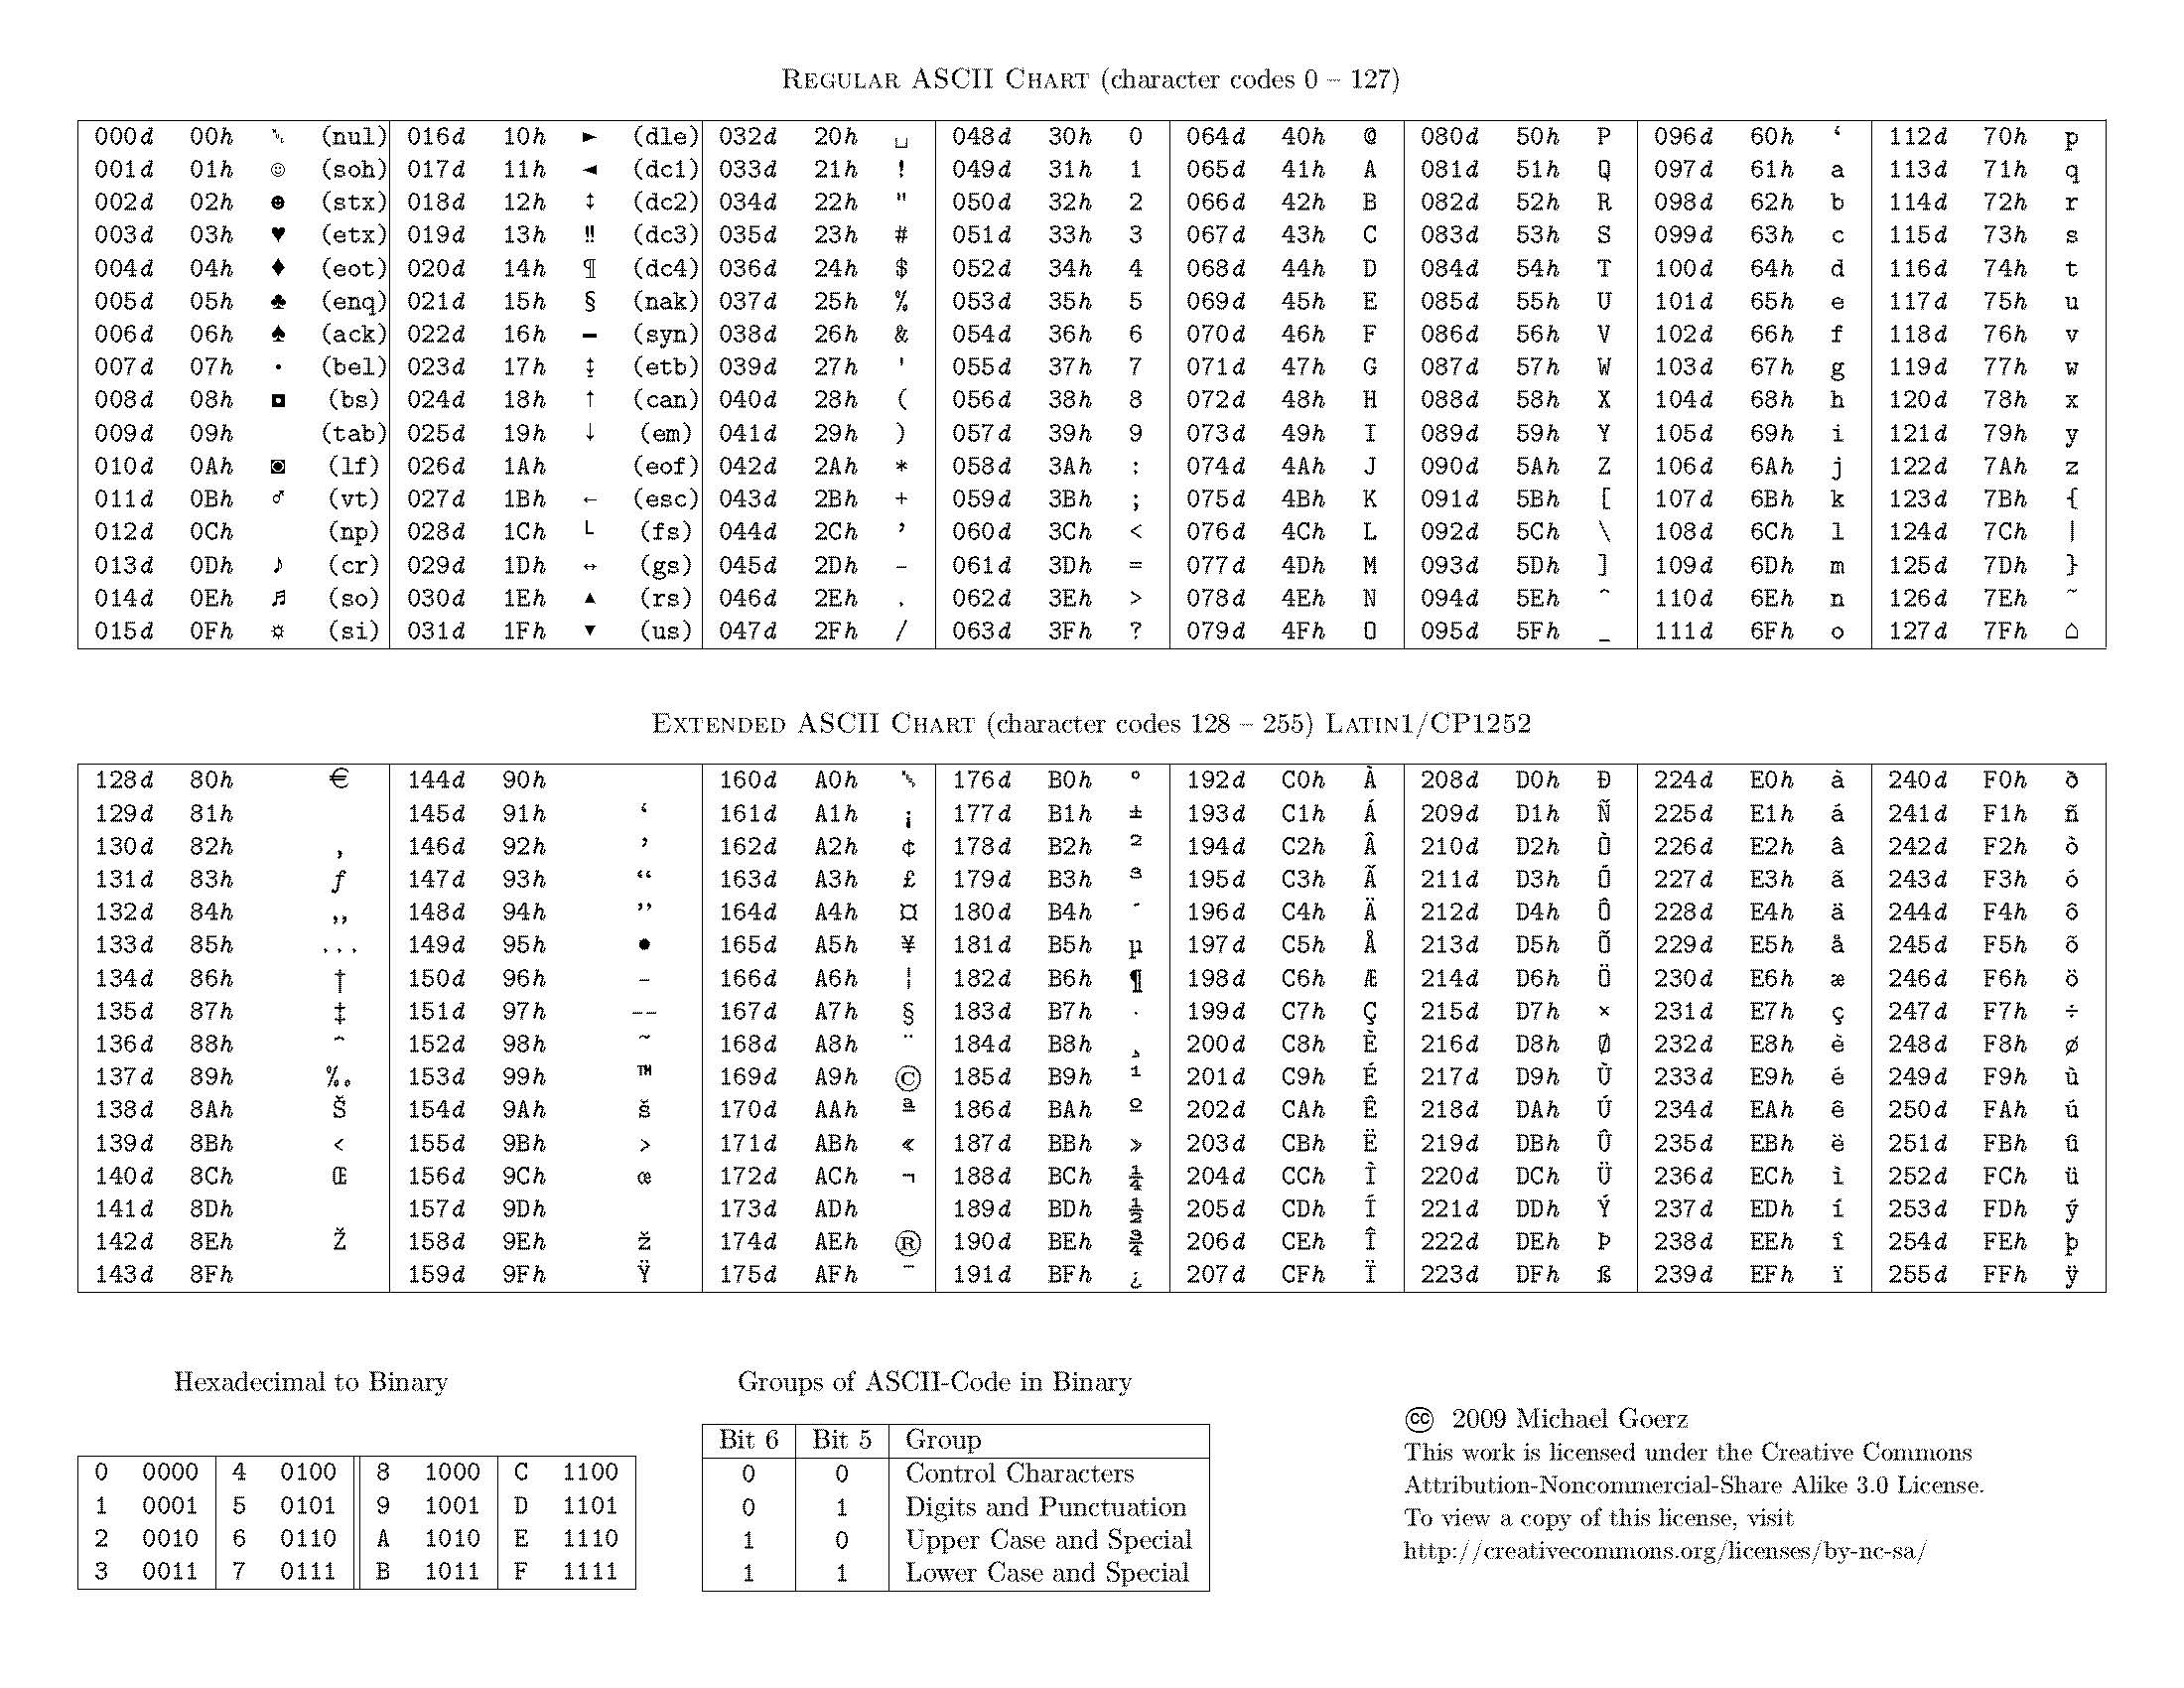
\includegraphics[width=0.8\textheight, angle=270]{ascii.jpg}
\end{center}
\end{document}
